\documentclass[french,a4paper,12pt]{article} 
\usepackage[utf8]{inputenc}
\usepackage[T1]{fontenc}
\usepackage[a4paper,left=2cm,right=2cm,top=2cm,bottom=2cm]{geometry}
\usepackage{mathtools}
\usepackage[french]{babel}
\usepackage{libertine}
\usepackage{blindtext}
\usepackage{babel}
\usepackage[pdftex]{graphicx}
\usepackage{lmodern}
\usepackage{url}
\setlength{\parindent}{0cm}
\setlength{\parskip}{1ex plus 0.5ex minus 0.2ex}
\newcommand{\hsp}{\hspace{20pt}}
\newcommand{\HRule}{\rule{\linewidth}{0.5mm}}
\selectlanguage{french}
\title{BP} % le titre de l'article
\author{Marina Cathy Beaujolais} 
\usepackage{caption,subcaption}
\tracinglostchars=2
\usepackage{iftex}
\pagestyle{plain}
\usepackage[authoryear]{natbib}
\ifTUTeX
  \usepackage{fontspec}
\else
  \usepackage[T1]{fontenc}
  \usepackage[utf8]{inputenc} % The default since 2018
  \DeclareUnicodeCharacter{200B}{{\hskip 0pt}}
\fi
\usepackage[]{tocbibind}
 \DeclareUnicodeCharacter{202F}{\,}

\begin{document}
\begin{titlepage}
  \begin{sffamily}
  \begin{center}
     
\includegraphics[scale=0.25]{logoulb.JPG}~\\[1.5cm]

    \textsc{\bfseries \LARGE Université Libre de Bruxelles }\\[0.5cm]
    \textsc{\Large Faculté de Lettres, Traduction et Communication}\\[6cm]

    % Title
    \HRule \\[0.4cm]
    { \huge \bfseries Sujet n°6 :​Évaluer les services​ d’une bibliothèque publique\\[0.4cm] }

    \HRule \\[4cm]
    % Author and supervisor
    \begin{minipage}{0.4\textwidth}
      \begin{flushleft} \large
        Aubert Marina \\
        Metango Kenfack Cathy \\
        Yepmou Beaujolais \\
        
      \end{flushleft}
    \end{minipage}
    \begin{minipage}{0.4\textwidth}
      \begin{flushright} \large
        \emph{Travail réalisé sous la direction de M. Christian Brouwer dans le cadre du cours Gestion des Bibliothèques (M-STIC-B420)} 
      \end{flushright}
    \end{minipage} \\ [2cm]

    \vfill

    % Bottom of the page
    {\large {} Année académique 2022-2023}

  \end{center}
  \end{sffamily}
\end{titlepage}


 %%fin de la parge de garde 
 \begin{center}
 \tableofcontents
 \end{center}
\newpage



\section{INTRODUCTION}




\newpage
\section{METHODOLOGIES}
Pour chaque étape du travail,  
Notre première étape a été de reformuler et de cadrer le thème du travail de groupe. 

\quad Nos questions de départ ont ainsi été formulées ainsi : Quels sont les services d'une bibliothèque publique ? Comment sont-ils évalués par rapport à leurs différents publics ? Comment les résultats de ces évaluations impactent-elles l'évolution de ces services ?\\
 
\subsection{Méthode de recherche​ et Équations de recherches}
\quad Premièrement, nous avons décidé de concentrer la recherche sur les sources en français et en anglais, les langues que nous maîtrisons. Deuxièmement, nous limiterons notre recherche bibliographique sur des publications académiques revues par des pairs, les plus robustes scientifiquement parlant. Troisièmement, nous viserons principalement la période située entre 2000 et 2022 : cette période de temps correspond à l’émergence des nouvelles technologies, et à la nécessité pour les bibliothèques publiques de s’y adapter. Elle nous permet donc d’évaluer à la fois les services traditionnels, présents depuis le début de la période, mais aussi les services directement liés aux nouvelles technologies, et enfin les nouveaux services, indirectement provoqués par cette nouvelle manière d'envisager le rôle des bibliothèques publiques. 

A partir de la bibliographie fournie, nous avons réalisé une première sélection de sources. Celle-ci a permis à Cathy et Beaujolais de réunir douze titres de périodiques et quinze livres. 

Parallèlement, Marina a élaboré l’équation de recherche, en français et en anglais, afin de lancer des recherches dans les instruments de travail de la bibliographie fournie :\textbf{ ((évalu* OR appréci* OR estim* OR examin*) AND services AND "bibliothèque* publique*") OR ((evalu* OR appr* OR estimat* OR valu* OR assess*) AND services AND "public librar*") }

Des niveaux différents de difficulté ont été rencontrés lors de l’utilisation de cette équation de recherche. La recherche dans la base de données @SIC n’a pas posé de difficultés, elle a délivré septante résultats. La recherche dans LISTA a généré trop de bruit, et Marina a dû activer des filtres limitants, et supprimer la recherche à des sujets équivalents ; finalement, cent soixante-et-un résultats ont été reçus. La recherche dans IFLA a résulté en un trop grand silence : la recherche a été lancée uniquement anglais, sans synonymes ; six résultats ont été délivrés.  

Les trois membres du groupe se sont réparti la sélection des sources parmi ces cent seize résultats. Finalement, notre corpus final a réuni cent-quarante-trois sources.  \\

\subsubsection{ Outils de gestion bibliographique : Zotero}
\quad Nous avons encodé notre corpus dans Zotero en préparation de la bibliographie de notre travail. Les sources ont été encodées en leur associant le type de services à évaluer (services traditionnels, services liés aux nouvelles technologies, nouveaux services), et les méthodologies d'évaluation à envisager (évaluations quantitatives (statistiques, enquêtes d'usage, enquêtes de satisfaction, méthode de Kantor, enquêtes de qualité), évaluations qualitatives (entretiens individuels, méthodes ethnographiques, écoute du personnel), indicateurs de performance). Nous avons élaboré ces mots-clés sur base du cours de Gestion des bibliothèques. Nous avons écarté les normes ISO qui évaluent l'impact des bibliothèques publiques, et non leurs services. 

En encodant notre corpus, Zotero a intégré de nouveaux mots-clés pour qualifier nos sources. Afin d’obtenir une vue hélicoptère de l’ensemble des sources, nous avons décidé de réaliser un travail d’affinage des mots-clés avant d’entrer dans l’analyse de nos sources pour l’état de l’art. Nous avons donc décidé de d’abord supprimer les mots clés liés aux situations géographiques, aux auteurs, et les doublons, de conserver les mots-clés qui décrivent des services ou des modes d'évaluation, et d’ensuite préparer un plan détaillé de l’état de l’art, avant de procéder à la rédaction. \citep{Gouyon François 2008}

C’est à ce stade que nous avons exposé notre démarche à la classe via une présentation Powerpoint ; ce dernier a été créé au fur-et-à-mesure de nos échanges sur la création de notre méthodologie et sur la répartition du travail. \\

\subsubsection{Référencement }
Nous nous sommes basés sur le cours elearning « What’s up doc » de l’Université virtuelle pour identifier le mode de référencement : (auteur, année)

\subsection{Répartition du travail entre les membres du groupe}
\quad Dès le début du projet, l’ensemble du travail a été divisé en quatre étapes : la constitution du corpus, la rédaction de l'analyse pour l’état de l’art, les études de cas, la finalisation. Pour chaque étape, le travail a été réparti de manière équitable entre les trois membres de l’équipe. \\

Chaque étape ou partie d’étape a été cadrée par une date d’échéance et des dates de rencontre, soit en bibliothèque, soit en visioconférence. \\

La rédaction est réalisée en latex avec Texmaker et Miktex, coordonnée via Github. Ce choix d’outil nous permet d’intégrer facilement le référencement de Zotero, et nous permet de nous entraîner pour la rédaction de nos prochaines rédactions pour le master. \\

\subsection{Planning d'exécution du Projet}
\begin{figure}[h]
\begin{center}

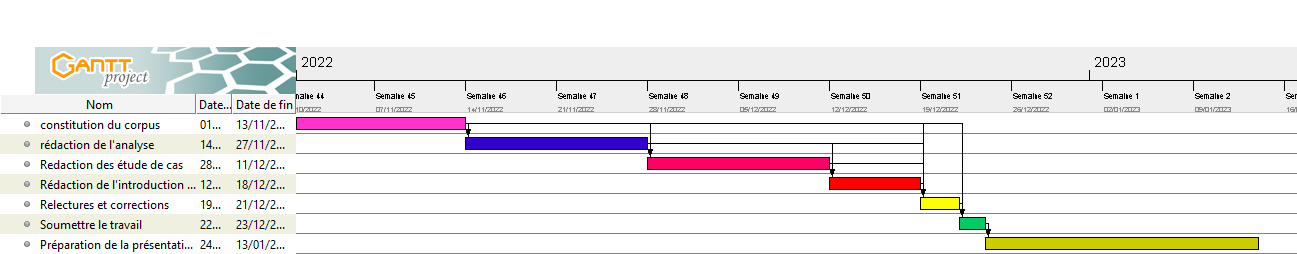
\includegraphics[scale=0.4]{document.PNG}
\caption{Planning d'exécution sujet 6}
\end{center}
\end{figure}




\newpage
\section{Etat de l'art}

\quad Lors du travail sur les mots-clés, Cathy s’est rendu compte que les sources avaient disparues de Zotero. Beaujolais et Marina ont réussi à récupérer les données perdues grâce à la sauvegarde automatique de Zotero. Ce sauvetage a pris plusieurs jours, a généré des sources en doublon à fusionner, et nous a imposé de réfléchir à une autre manière de réaliser l’Etat de l'art : nous avons renoncé à supprimer les mots-clés de Zotero, et estimé que nous allions chacune et chacun consulter les mots-clés en fonction de nos services à évaluer. 
Cathy se concentre sur l’évaluation des services traditionnels, Beaujolais sur l’évaluation des services liés aux nouvelles technologies, et Marina sur l’évaluation des nouveaux services.\\
\quad 



\subsection{Evaluation des services traditionnels}


\quad les gestion dune bibliothèque recouvre plusieurs types de services. cette partie partie traitera des services traditionnelles. parmis ces services , nous avons Accueil et inscription des utilisateurs, Consultation de documents imprimés, Promotion de la lecture, Prêt de documents ,Consultation de documents électroniques ,Aide à la recherche d’information ,Site web d’information.  


\subsubsection{Objectifs des services traditionnelles} \citep{Gouyon}

\quad avant dévaluer ces service nous devons dabord présenter ses objectifs.

\quad pour le service  d'animation, la collection ne semble pas basique.  les employés doivent et peuvent adhérer à des clubs locaux. Promouvoir régulièrement les activités de la bibliothèque. Concernant le matériel, Des installations adéquates et accessibles et des moyens de communication efficaces sont nécessaires. 

\quad Pour fonctionner comme service d'information et de documentation, la collection doit contenir des références générales et fournir des données précises sur les services et les associations. Le personnel doit être formé aux techniques de documentation, à la connaissance des services et ressources communautaires, du répertoire et de la manière dont le répertoire est organisé et maintenu. L'appareil doit être facilement accessible et offrir un espace de travail et de consultation suffisant.  

\quad Pour fonctionner comme un bureau d'aide à l'apprentissage, la collection doit contenir toutes sortes de documents, en particulier des documents de référence, du niveau d'enseignement approprié. Le dispositif doit être accessible, notamment par l'établissement d'enseignement, offrir un espace de travail individuel, fournir des outils informatiques et pouvoir travailler dans un laps de temps raisonnable. 
 \quad En raison de son rôle de centre d'auto formation, la collection doit comprendre un large éventail de ressources documentaires adaptées à tous les niveaux et à toutes les matières. Le personnel doit avoir des connaissances pédagogiques et être familiarisé avec les principes généraux de formation et les possibilités de formation locales. L'équipement doit être facile à utiliser, avoir une signalétique efficace et avoir une surface de travail qui garantit un certain degré de silence. Doit fonctionner selon une amplitude de temps suffisante. La tâche de livrer une collection populaire nécessite de diversifier la collection avec différents supports avec suffisamment de spécimens et des documents récents. Le Le personnel doit avoir une bonne compréhension des attentes du public, des versions "grand public" et des best-sellers. La conception en libre accès doit encourager la navigation, la signalisation doit être efficace, les étagères doivent être facilement accessibles, des chaises doivent être fournies et les bibliothèques doivent être faciles d'accès. 


\quad Son rôle de centre de référence et d'information nécessite des collections répondant à tous les besoins d'information, des documents adaptés à tous les niveaux de lecture, des références volumineuses avec bases de données, accès Internet, revues et dossiers d'information. Un personnel formé à l'utilisation des outils de référence et expérimenté dans la revue de documents doit être disponible. L'équipement doit contenir une zone visible et bien délimitée pour effectuer des services de renseignements et des recherches en ligne. 
Après cette présentation générale des moyens dont la bibliothèque doit s’assurer de pouvoir disposer pour remplir ses objectifs, il nous reste maintenant à présenter comment, concrètement, la bibliothèque peut évaluer l’efficacité et l’efficience de ces services. 



\subsubsection{Mesure de l’activité et du service rendu} \citep{Gouyon}

\quad  La mesure de l'activité et de la performance de la bibliothèque, notamment le degré d'atteinte des objectifs fixés par la bibliothèque et l'évaluation des conditions dans lesquelles ce résultat est atteint, s'effectue principalement à l'aide de métriques. Par conséquent, lorsque nous parlons d'indicateurs et de la manière de les utiliser, nous allons d'abord découvrir de quoi il s'agit. Les bibliothèques ont deux normes \textit{ISO 2789 et ISO 11620} pour mesurer leurs activités, qui fournissent un ensemble d'indicateurs, donc la deuxième étape se concentrera sur ces normes. Voyons maintenant comment A.L.A. fonctionne dans la deuxième pièce. Il offre aux bibliothèques l'occasion de mesurer leurs activités et d'évaluer les services qu'elles fournissent. 

\subsubsection{Indicateur de performance } \citep{Gouyon}

\quad Les indicateurs sont liés aux objectifs de la bibliothèque. mais comme nous Comme nous l'avons vu, ce ne sont pas des buts en soi. Un outil permettant de calculer et d'afficher le niveau de performance de Mesurer les résultats des bibliothèques et des activités spécifiques Référence à un objectif défini ou à un ensemble d'objectifs. Les indicateurs pour leur construction sont basés sur des données statistiques. Cependant, ils diffèrent en ce qu'ils représentent une interprétation de ces données. 
référence croisée ou comparaison ou comparaison de données brutes, pour la plupart différentes relation entre eux. Donc le nombre d'abonnés à la bibliothèque est la date statistiques. La population totale desservie variera. En signalant D'abord ces données, puis les indicateurs, les taux de scolarisation ou Le taux d'impact, qui mesure la proportion de la population qui doit être desservie 
Inscrivez-vous à la bibliothèque. Donc, pour construire une métrique, vous devez collecter des données dans un but précis pour savoir ce que vous essayez de mesurer et pourquoi vous voulez le mesurer. 
 
 \subsubsection{Evaluation par la methode de kantor}\citep{LapèlerieFrançois1994}

\quad En 1976, Paul B. Kantor a développé une méthode simple et peu coûteuse pour évaluer les bibliothèques. Sur la base de nos recherches d'utilisateurs, nous pouvons vous aider à découvrir pourquoi le livre que vous recherchez n'est pas réellement disponible ou si vous pensez qu'il n'est pas disponible. Cette méthode a ensuite été étendue aux magazines également. Kantor répertorie et illustre les quatre principales causes de panne de disque. Ces causes nous permettent d'évaluer l'efficacité des différents services offerts par la bibliothèque. Nous examinons ensuite leur importance relative et leurs rôles, ainsi que les solutions possibles.

\quad L'efficacité de la bibliothèque est mesurée par un critère très simple. Certains lecteurs ont besoin de certains documents à certains moments. Les bibliothèques doivent se conformer à cette demande. Selon que ce lecteur trouve ou non quelque chose sur le site, il juge de la qualité supposée de la bibliothèque. Ce jugement peut être nuancé a le mérite de refléter fidèlement la situation dans laquelle se trouve le lecteur. Il est à la fois négatif et permet aux bibliothécaires d'évaluer plus positivement la performance de la bibliothèque. Les bibliothécaires ne jugent pas les cas individuels qui peuvent être considérés comme des exceptions. Il a tendance à rendre des verdicts globaux sur son entreprise. La bibliothèque satisfait x pour cent de ses lecteurs, et le bibliothécaire peut être satisfait (ou mécontent) d'atteindre son quota. A l'inverse, les lecteurs qui n'ont pas pu trouver ce dont ils ont besoin ne sont pas contents de la malchance de se retrouver dans la "minorité" que les bibliothèques ne peuvent satisfaire. Cependant, c'est cette notation par les usagers qui est à la base du reflet de la disponibilité des documents en bibliothèque et donc de la qualité du service.


\quad En revanche, si une bibliothèque peut répondre à tous les besoins de ses lecteurs avec un taux d'erreur très faible voire nul, soit elle achètera tout ce qui paraît impossible, soit elle n'utilisera que le bien pour un service particulier. Vous pouvez attendre de lui sans demander plus. Connaître ce que vous pouvez appeler le taux d'échec est inhérent à chaque bibliothèque. Par conséquent, il est logique de fonder la disponibilité d'un document dans une bibliothèque, c'est-à-dire son efficacité sur l'approche du lecteur par rapport au document. Aligner la bibliothèque avec son rôle de base. Un service pour les lecteurs qui rend la documentation facilement accessible. Les bibliothécaires peuvent également considérer la bibliothéconomie comme : La bibliothéconomie est un ensemble de techniques qui jouent un rôle fondamental dans les bibliothèques, et non l'inverse. Les indices traditionnels dérivés des statistiques de fonctions globales sont très primitifs. Ils rétrécissent le champ de la recherche, surestiment constamment l'efficacité des bibliothèques et ne font que confirmer ce qui est déjà connu.

 \quad Cette étude de la satisfaction ou de l'insatisfaction des lecteurs a fait l'objet de nombreuses publications conduisant à l'élaboration d'indicateurs permettant d'améliorer la performance des bibliothèques.
 
\subsubsection{Les bibliothèques en tant que services publics d'information} \citep{LapèlerieFrançois1994}

 \quad Les bibliothèques sont des services publics d'information. Ce service public a certains coûts qui lui sont associés. La recherche américaine sur l'accessibilité ignore délibérément le côté économique du problème parce qu'il ne fait pas partie du problème. Cependant, les fonctions de la bibliothèque doivent être remplies à un certain prix, elles ne peuvent donc pas être complètement ignorées. Les bibliothèques doivent optimiser leur utilisation des crédits pour atteindre le coût marginal le plus bas possible pour chaque utilisation supplémentaire de leurs services. Cet aspect doit être intégré dans la mesure du possible, car il peut influencer les décisions à prendre. En effet, dans certains cas il y a deux solutions possibles pour résoudre la panne. L'un est fonctionnel (changement de règles de fonctionnement, donc pas de surcoût) et l'autre matériel (tâches achetées et/ou nouvelles, donc surcoût).
 
 \quad \citep{LapèlerieFrançois1994} Les bibliothèques agissent comme des services publics au service du savoir. Il participe au transfert de connaissances. Comment mesurez-vous le transfert de connaissances ? Il ne peut pas être mesuré en soi, nous nous limitons donc à observer des événements concrets liés à cet objectif. Un guide important est la satisfaction du lecteur. Les lecteurs effectuent certains gestes pour trouver ce dont ils ont besoin. Ces activités (parcours de dossiers, recherche de documents dans les rayons, prêt, etc.) reflètent la recherche de connaissances, et l'exploration des connaissances est la représentation la plus précise et la plus objective de la contribution de la bibliothèque à cet objectif fondamental, ce qui conduit à la détermination de mesures réalistes. On pense donc que répondre à la demande améliore l'efficacité des bibliothèques dans leur rôle de partage des connaissances. 
 




\subsection{Évaluation des services liés aux nouvelles technologies}

\quad D'après LAROUSSE, le terme Nouvelles technologies signifie :\textit{ moyens matériels et organisations structurelles qui mettent en œuvre les découvertes et les applications scientifiques les plus récentes. (On dit aussi haute(s) technologie(s), technologie(s) de pointe, technologie(s) avancée(s).)}\\

\quad De nos jours, les bibliothèques connaissent des grandes mutations dues au développement des technologies de l'information et de la communication. Ces mutations affectent tant les services offerts par les bibliothèques, mais aussi la fonction du Bibliothécaire. En effet, Les fonds électroniques, des espaces de lecture numériques (à travers un ordinateur), La dématérialisation des sources d'information en passant par la numérisation des collections, Soulève des interrogations qui selon Imad Salech \textit{<<Gravite autour de la migration annoncée du matériel vers l'immatériel, du réel vers le virtuel et de l'analogique vers le numérique >>}\citep{saleh_bibliotheques_2009}. Tout au long de cette section, nous étudierons l’enjeux  des nouvelles technologies  sur les bibliothèque publique d’une part, d’autre part nous parlerons de l’importance de l’évaluation de cet outils  et enfin de comment sont-il évalué ?

\subsubsection{Enjeux} 

 
 \quad L’enjeu de l'utilisation de nouvelles Technologies de l'information et de la communication au sein des bibliothèques publiques est certes varié en fonction des besoins de la population desservie car il est important de souligner que le numérique à une fonction principale de soutenir ou de facilité l'accès à des services au sein de la bibliothèque. Que ça soit par les services de lecture assistée par Ordinateur d'une part, d’autre part de la télé documentation (accès à distance des documents) et de la numérisation des collections ou des espaces et appareils adaptés pour que les utilisateurs puissent consulter les collections numériques et faire des recherches (ordinateur, accès à internet, casque audio, Vidéoprojecteur, écran de projection), L'enjeu ici du point de vue global est de satisfaire le public en répondant de façon numérique à ses exigences. En outre, il est aussi important de rappeler que plus une bibliothèque est visitée Plus les services offerts par cette dernière répondent aux besoins du public cible, d'où l'importance d'un accompagnement dans la prise en main des nouveaux outils mis à leur disposition tant pour le Bibliothécaire acteur d'une part, du transfert de compétences ou de formation des usagers, D'autre part maillon fort de l'utilisation de ces outils pour la bonne marche de la bibliothèque. En d’autres termes, il ne faut pas faire du numérique. Pour le numérique mais pour répondre à un besoin ou un projet spécifique.\\
En ce qui concerne les bibliothèques, Comme le dit Camille Rondot en parlant de Gérard Regimbeau, l'association entre ces deux mondes (des bibliothèques et numériques) crée du sens dans la mesure où elles permettent de construire un lieu structuré dans lequel se rassemble \textit{<< Tout le savoir du monde >> }dans un imaginaire de complétude\citep{rondot_bibliotheques_2022}.Étant donné leurs rôles d’accès à la culture et leurs agissements en matière de formation, les bibliothèques publiques jouent un rôle particulier pour ce qui du développement des compétences numériques par leurs publics, diffusion de contenus sur internet et d’inclusion numérique. Par ailleurs, toutes les bibliothèques publiques ne sont pas capables de nos jours d’assurer ces rôles car : 
\begin{enumerate}
\item[•] Pour certaines bibliothèques publiques dont les budgets sont relativement bas n’ont pas de matériels et connexion adéquate.
\item[•] Pour d’autres, cela est non seulement dû la non-maîtrise des outils numériques par le bibliothécaire, mais aussi par l’intérêt que ce dernier n’appréhende pas. D’où la nécessité d’une formation et suivi après le déploiement d’une telle solution.
\end{enumerate} 
\quad La mise en place des normes et statistiques afin d'évaluer l’impact des services liés aux technologies au sein des bibliothèques publiques sont donc important.\\

\subsubsection{Normes d'évaluations\citep{young1998evaluation} }

\quad Une norme, du latin norma « équerre, règle », désigne un état habituellement répandu, moyen, considéré le plus souvent comme une règle à suivre. \\
\quad La mise en place d’une politique d’évaluation permet de mettre en lumière l’impact des technologies de l’information et de la communication sur certains services et fonctionnement de la bibliothèque. 
Selon Peter R. Young, \textit{<<Les relevés d'utilisation d'Internet et du World Wide Web offrent la possibilité d'identifier les usages locaux et à distance des supports et services électroniques, grâce à des informations "système">>\citep{young1998evaluation}}. Afin de suivre statistiquement la piste des utilisateurs, établir leurs profils et identifier les besoins spécifiques des usagers, il est nécessaire d’employer les professionnels du métier du numérique pour évaluer le "qui utilise quelles ressources ?". Ainsi, l’évaluation de l’usage des services lié aux nouvelles technologies donne d’une part des rapports détaillés sur l’usage des services fournis ou non par la bibliothèque (qui peut être par exemple un type de collection, donc la bibliothèque ne possède pas), d’autre part elle fournit les besoins ou attentes des utilisateurs et leurs satisfactions. \\
\quad En outre, pour mesurer l’impact des activités liées aux nouvelles technologies, les bibliothèques ont développé des méthodes quantitatives classiques fournissant des rapports qualitatifs sur l’efficacité et le gain de celle-ci afin de répondre a l’exigence du public cible.\\





\subsubsection{Approches de l'évaluation}
\quad Elles identifient de fond en comble les besoins spécifiques des usagers et du fonctionnement bibliothèque à travers les services liés aux nouvelles technologies. Elles sont fondées sur les approches suivantes. 

\begin{enumerate}
\item[•]L’approche basée sur transactions : elle utilise les techniques d’enquête de la méthode quantitative d’évaluation des services pour mesurer entre-autre les périodes interactives et la quantité d'informations reçue rapportée au nombre de terminaux connecté 
\item[•]L’approche basée sur le temps de connexion : elle vise à évaluer la charge des équipements (serveur, wifi, etc.) pendant les périodes de pointe ou les horaires de fonctionnement en utilisant la méthode statistique.
\item[•]L'approche basée sur les dépenses : elle vise à évaluer les coûts (charge) due aux équipements informatiques, logiciel, internet, licence, etc.
\item[•]L’approche basée sur l’utilisation : vise à identifier et à améliorer les besoins grâce à la méthode statistique et d'enquête ou de sondage (d’usage simultané des ressources numériques ou indicateur de disponibilité des places de travail, de satisfaction, de qualité et nombre de recherches ayant abouti par l’usager, etc.).
\end{enumerate}




\subsubsection{Difficulté de l'évaluation}
\quad Cette étude est issue de la Commission Nationale Américaine Sur Les Bibliothèques Et Les Sciences De L’information, elle décrit les difficultés rencontrées par les bibliothèques en ce qui concerne l’évaluation des services numériques à cause de l’évolution rapide des technologies de l’information et de la communication \citep{bertot_1996}: 

\begin{enumerate}
\item[•]L’élaboration des normes sur les charges fonctionnelle et d’investissement liée aux nouvelles technologies (équipement informatique, compatibilité logicielle, licence, modem internet, etc.)
\item[•]L’élaboration des normes communes destinée à mesurer l’impact des actions collaboratif et collaboratif entre bibliothèques elle-même et entre celles-ci et les autres institutions pour la fourniture de supports et services électroniques.
\item[•]Problème de compatibilité entre systèmes et nouvelles versions de logiciel ou logiciel existante et nouvelle version de système due aux mutations technologiques.
\item[•]Difficulté à évaluer quantitativement les produits et objet multisupports dû à l’absence d’un cadre normatif.
\item[•]Difficulté à suivre l’évolution des coûts et pratiques commerciales chez les éditeurs de contenus électronique et prestataires de service en réseau.\\

\end{enumerate}



\subsection{Evaluation des nouveaux services}

\quad Outre l’emprunt et l’utilisation des ressources numériques de la bibliothèque, Claude Poissenot\citep{lanouvellebibliotheque2009} identifie des nouveaux services des bibliothèques publiques : la mise à disposition des espaces pour un usage studieux (hors recherche documentaire), l’accès à la culture et au divertissement, l’utilisation des espaces pour se rencontrer. 

\subsubsection{L’usage studieux de la bibliothèque }

\quad Claude Poissenot évoque notamment un aménagement de l’espace centré sur les besoins des différents publics, et la mise en place de nouveaux services adaptés :  soutien scolaire, aide aux devoirs, et une offre documentaire parascolaire et orientée vers la formation continue. 

Désormais, les étudiants et les lycéens viennent étudier, seuls ou en groupes, dans les bibliothèques publiques.  

\quad A la Bibliothèque publique d’information du Centre Pompidou à Paris\citep{etudiants2014}, une analyse des enquêtes de fréquentation réalisées à partir de 2003 a permis de préciser les profils et les usages : 

“Les enquêtes de fréquentation générale de 2003, 2006 et 2009 ont été menées selon la technique du sondage aléatoire. Cette technique consiste à interroger, à intervalle régulier, des usagers sortant définitivement de la bibliothèque. Il s’agit là d’une méthode de passation que l’on dit par « voie administrée », contrairement à la voie auto-administrée qui consiste à laisser le répondant remplir tout seul son questionnaire. En novembre 2003, de même qu’en novembre 2009, le pas de tirage choisi était de 3 (autrement dit : 1 personne sortante sur 3 était systématiquement interrogée) ; en novembre 2006, le pas, d’abord fixé à 4, dût être réévalué à 6 et 8.” 

Les étudiants fréquentent la Bpi notamment à cause de ses larges plages d’ouverture. Cependant, les étudiants avouent préférer parfois d’autres institutions, notamment à cause de la durée d’attente. Les étudiants en Sciences, techniques et santé sont les plus nombreux à fréquenter la bibliothèque, notamment durant les trois premières années de ses études. Ils sont particulièrement indépendants, c’est-à-dire qu’ils ne s’adressent pas (ou peu) aux bibliothécaires. Ils déclarent « se débrouiller seuls » en particulier en menant des recherches en ligne sur Internet. 

\quad La Bibliothèque publique d’information du Centre Pompidou à Paris a également évalué l’usage des espaces par des lycéens qui y préparaient leur baccalauréat\citep{lyceens2010}. 

Cette évaluation a été réalisée sur base de 14 entretiens semi-directifs, 1 focus group (entretien collectif) et 9 séances d’observation ont été menés entre mai et juillet 2010. Les personnes enquêtées ont été recrutées dans l’ensemble des espaces de la bibliothèque. 

Les résultats montrent que les lycéens utilisent les espaces d’étude de la bibliothèque pour s’investir - tant sur le plan symbolique que pratique - dans un travail de révision scolaire intensive tout en profitant d’un anonymat relatif et d’une sociabilité studieuse. Leur usage de l’espace et des collections ressemble fortement à celui des étudiants. Ils apprennent ainsi les normes comportementales attendues dans une bibliothèque d’étude, et plus largement celles requises pour les études supérieures. Ils opèrent ainsi un important processus de socialisation aux études supérieures.  

L’étude précise : “L’installation dans une grande bibliothèque pour réviser les épreuves du baccalauréat constitue une sorte de rite de passage au cours d’une phase critique de l’existence : plus exactement un phase intermédiaire où l’on quitte le lycée et ses contraintes (ie le statut d’enfant), l’environnement proche, dans l’espoir d’accéder à un autre niveau (les études supérieures, le statut de jeune adulte). La bibliothèque participe donc d’un mouvement de coupure et de transformation qui va au-delà des seules révisions.“ 

Par ailleurs, ils empruntent très peu de ressources documentaires, hormis les annales du baccalauréat des années précédentes mise à disposition, malgré le dispositif d’information, qu’ils jugent négativement. L'enquête leur a permis de suggérer de nombreuses propositions au sujet des ressources, des documents d’information, des espaces de la bibliothèque et des personnels. 

\subsubsection{L’accès à la culture et au divertissement}

\quad Claude Poissenot  propose la bibliothèque pour se détendre via son implantation dans des zones de passage ou d’activités, via l’accès à un moment de “Rendez-vous avec soi”, ou simplement un moment de détente. 

La Bibliothèque publique d’information du Centre Pompidou à Paris propose justement ses services au sein du complexe culturel Pompidou. Ce dernier dispose également de musées et d’espaces d’exposition permanente ou temporaire, de salles pour divers événements (spectacles, concerts, cinéma, conférences, festivals, soirées), pour tous les publics. Il propose des offres de services spécifiques pour les écoles et pour les jeunes\citep{expositions2012}. 

\quad La Bibliothèque publique d’information du Centre Pompidou a réalisé en 2012 une enquête sur la perception des expositions organisées dans ses espaces de lecture 5, via une enquête par observations et des entretiens semi-directifs. Cette évaluation a été conçue dans le cadre de quatre expositions, offrant autant de dispositifs différents : Archipel (dispositif interactif d’écoute et de découverte de musiques contemporaines) ; Presse-citron (exposition de reproductions de dessins de presse) ; Éditeurs, les lois du métier (exposition thématique, présentant des originaux sous vitrine et un rédactionnel important) ; Spiegelman (exposition monographique essentiellement composée d’œuvres originales de l’auteur de Maus). 

Les résultats de l’enquête montrent que les publics souhaitent s’approprier des expositions qui produisent du sens et s’ancrent dans un monde vécu. La visite guidée leur permet de bénéficier des clés de lecture utiles pour décrypter les œuvres, elle permet tout à la fois de s’ouvrir à l’inconnu et de trouver des prises nouvelles. Certains visiteurs apprécient d’être entièrement « pris en main » par le conférencier, tandis que d’autres souhaitent seulement être orientés et recevoir des informations leur permettant d'envisager et de visiter l’exposition individuellement, à leur rythme. 

\quad En 2017, une évaluation a également été commandée en marge de l’exposition « Gaston, au-delà de Lagaffe »\citep{gaston2019}. Elle a été confiée à Fanny Ankri, élève bibliothécaire de l’Enssib, dans le cadre de sa formation initiale de bibliothécaire d’état, et a été constituée de 44 entretiens semi-directifs, individuels ou collectifs, menés avant, pendant ou après la visite de l’exposition.  

Les résultats révèlent que les visiteurs déclarent très majoritairement avoir pris beaucoup de plaisir à visiter l’exposition Gaston. Néanmoins, pour certains sur la lecture des planches s'est avérée difficile : hauteur des accrochages, densité et format de l’exposition, emplacement des vidéos.  

\subsubsection{Lieu de rencontre}

\quad A contrario de l’usage historique des bibliothèques comme un lieu silencieux, Claude Poissenot  décrit les nouvelles bibliothèques publiques comme espace pour tisser des liens et socialiser, entre utilisatrices et utilisateurs, mais aussi avec le personnel et via des animations. 

Grâce au réservoir de connaissances des bibliothèques publiques, de nouveaux espaces informationnels se créent, notamment par la mise en scène de l’information 7. 

\textbf{Ateliers « makerspaces »}

\quad Le mouvement des makers\citep{makers2020} est à l’origine une initiative de Make magazine pour célébrer la culture américaine du « faire soi-même », dès 2005. Les ateliers « makerspaces » proposaient des formules très diverses d’animations, toutes basées sur la rencontre autour d’outils, de projets, d’accompagnateurs et d’expertise. Ils servent à fabriquer. En 2015, Barack Obama a proclamé le lancement de la Semaine nationale de la fabrication, pour attirer l’attention sur le mouvement des « makers » et l’apprentissage des STEM (Sciences, Technologie, Ingéniérie, Mathématiques ). Partout dans le monde, des bibliothèques audacieuses ont ajouté des « makerspaces » à leurs services. 

A la bibliothèque des sciences de l’université Clarion de Pennsylvanie (Etats-Unis), une étude qualitative a été réalisée auprès de 21 utilisateurs de 2 bibliothèques équipées de « makerspaces ». Les méthodes d’évaluation incluaient les entretiens individuels, des observations, des photovoix, des focus groups. 

Les résultats montrent que ce nouveau service a étendu le modèle des pratiques d'information quotidiennes, et a comblé les lacunes de la littérature sur le comportement et les pratiques d'information des jeunes. Ils confirment que les conceptualisations des pratiques informationnelles sont un aspect indissociable et naturel des pratiques sociales et des événements de la vie quotidienne des individus. 

\textbf{Services sociaux}

\quad En 1991, l’American Library Association a attiré l’attention sur les besoins d’accès à la lecture des sans-abrs et des personnes socioéconomiquement désavantagées\citep{servicessociaux2008}. Depuis, les services sociaux interviennent pour améliorer les services aux pauvres et la formation des bibliothécaires.  

Certaines bibliothèques ont ainsi formé des équipes de sensibilisation spécialisées dans les besoins des sans-abris. ; d'autres ont développé des répertoires de ressources ; d'autres encore ont établi des partenariats formels avec des services sociaux et des agences gouvernementales. 
 
Une enquête ethnographique qualitative a été réalisée dans les bibliothèques publiques canadiennes en 2008 pour évaluer les auto-perceptions des travailleurs sociaux et les opinions de leurs collègues sur ce travail. Elle s’est basée sur des entretiens individuels et des données de groupes de discussion de trois sites de bibliothèques publiques à travers le pays. 

Les résultats indiquent que l'appel à adopter un changement de culture dans la bibliothèque pour mieux servir les populations vulnérables est tempéré par des défis liés à l'efficacité des formations du personnel, à la clarté du protocole et de la procédure, aux lacunes dans la supervision et à l'utilisation de l'espace. 

 

 







\subsection{Méthodes d'évaluation}

\subsubsection{Méthodes quantitatives}


\subsubsection{Méthodes qualitatives}

\subsubsection{Methode kantor }

\quad Une enquête auprès des usagers des bibliothèques identifie les raisons pour lesquelles les lecteurs n'ont pas trouvé la cause par le nom de l'auteur ou le titre du document (livre ou revue) et, si possible, le pourcentage correspondant. Aucune recherche n'a été effectuée sur la recherche thématique.
Il est certainement utile de le faire pour mesurer objectivement l'efficacité du reporting par sujet. En indiquant la cause de l'erreur, vous devriez pouvoir demander une amélioration même si vous ne la trouvez pas. 
\quad C'est kantor qui a cherché à développer un modèle mathématique de la disponibilité immédiate des documents, basé sur des recherches menées dans sa bibliothèque. De plus, nous tentons de déterminer une mesure de la satisfaction des utilisateurs appelée TCT/P, ou Total Contact Time per Potential user, divisé en huit paramètres. Kanter est à l'origine de l'étude de la disponibilité des documents dans les bibliothèques à travers sa méthodologie et les modèles mathématiques qu'il a développés.

 \paragraph{Principes}  
 
 \quad L'objectif est de comprendre pourquoi les lecteurs ne trouvent pas les documents qu'ils recherchent dans la bibliothèque. la méthode est facile. Un nombre statistiquement significatif de lecteurs est approché lorsque les lecteurs recherchent des documents en libre accès. Un formulaire préparé à cet effet vous demande d'inscrire l'auteur, le titre et la cote du document recherché. Les lecteurs utilisent ce formulaire pour enregistrer leurs résultats de recherche, s'ils ont trouvé le document, leurs commentaires s'ils ne l'ont pas trouvé et leurs commentaires. Le chercheur doit vérifier l'exactitude matérielle des données détenues par le lecteur, l'exactitude de la recherche menée par le lecteur, ordonner les données brutes et créer statistiquement.
 
 \paragraph{évaluation}  
 
 \begin{enumerate}
  \item[•]  Évaluation du  nombre de visites en fonction de la population desservie : le Retrait est fait au comptoir d'entrée de la bibliothèque. Les résultats sont des indicateurs de l'adéquation des heures d'ouverture, des communications de la bibliothèque et de la pertinence des fonds par rapport aux besoins de la population. Une approche plus précise de cet indicateur doit être en mesure de déterminer les heures de pointe, les groupes de population les plus représentés dans les bibliothèques et si le nombre d'employés de la fonction publique est adéquat. Oui. Cette mesure devrait être liée au taux de distribution des documents ( taux de rotation). 
  
 \item[•] Évaluation du Tarif dinscription   : Les enquêtes sont menées via SIGB. La fiabilité de cet indicateur nécessite que le registre des inscrits soit tenu à jour. Cet indicateur montre la qualité de la communication menée par la bibliothèque et la pertinence des collections par rapport aux besoins de la population desservie. Plus généralement, il renseigne sur la satisfaction de la population desservie à l'égard des services offerts par la bibliothèque. 
 
  \item[•]evaluation du  nombre de prêts en fonction de la population desservie les enquêtes sont menées via SIGB. Cet indicateur renseigne sur la pertinence de procédures spécifiques (telles que les périodes de prêt), le traitement des collections et leur approche par les besoins, les communications de la bibliothèque et les heures de travail. Une approche plus détaillée de cet indicateur conduit à travailler avec des segments spécifiques de la collection. Cette mesure doit être liée au chiffre d'affaires pour déterminer si la collection est bien développée, pertinente et à jour. 
  
   \item[•]  le Taux de rotation : le recueil se fait via le SIGB. Cet indicateur peut avoir plusieurs significations. S’il est haut cela peut signifier que la collection est sous dimension 
Née, ou bien qu’elle est très intéressante pour la population à desservir. S’il est bas, cela peut signifier que tout ou partie de la collection est très spécialisée, peu populaire, obsolète où inappropriée. Il renseigne également sur la nécessité d’un désherbage, sur la qualité de la présentation et de la disposition des documents ainsi que sur la pertinence de l’amplitude horaire. 

\item[•]  Nombre de références trouvées par rapport au nombre de références recherchées : La recherche se fait par la recherche. Je suis intéressé par le nombre de références trouvées par titre, auteur et sujet. Cet indicateur permet de mesurer la pertinence des collections par rapport aux besoins de la population desservie, la disponibilité des documents et les services rendus. En revanche, il ne dit rien sur les causes des échecs de recherche : collecte insuffisante, procédures inadaptées (ex : durée de prêt trop longue), ou recherches difficiles pour les utilisateurs. En fait, c'est une mesure de satisfaction. Cela permet aux bibliothèques de connaître la pertinence de leur fonds (nombre de titres et d'exemplaires) et leurs processus (stockage, catalogage, durée de prêt, etc.). 

\end{enumerate}

\newpage
\section{Etude de cas et retour d'expérience}
\quad Parallèlement, nous avons entamé la réflexion des choix d’études de cas. Avec les informations glanées lors des présentations des autres groupes de la classe, nous avons envisagé autrement les études de cas possibles : nous avons augmenté la diversité des cas.\\ 

Marina va étudier le cas de la Cité des métiers de Bruxelles, une bibliothèque publique spécialisée dans l’orientation professionnelle. Celle-ci se situe au rez-de-chaussée de la tour Astro, à la station de métro Madou, dans laquelle se trouvent les bureaux centraux d’Actiris.

.................................\\
\subsection{Etude de Cas 1:Cité des métiers de Bruxelles }
\quad La Cité des métiers de Bruxelles est un espace regroupant une bibliothèque spécialisée dans la formation et la recherche d'emploi, des ordinateurs et tablettes équipés pour la recherche d'emploi, des animations collectives, du conseil d'orientation professionnelle. C'est grâce à l'exposé du cours que Marina s'est rendu compte qu'il s'agissait d'une bibliothèque « nouvelle génération ». Marina travaille comme digital expert pour Bruxelles Formation, et est notamment en charge du site web de la Cité des métiers de Bruxelles. Elle dispose donc de tous les contacts sur le terrain pour réaliser cette étude de cas.
\begin{figure}[h]
\begin{center}

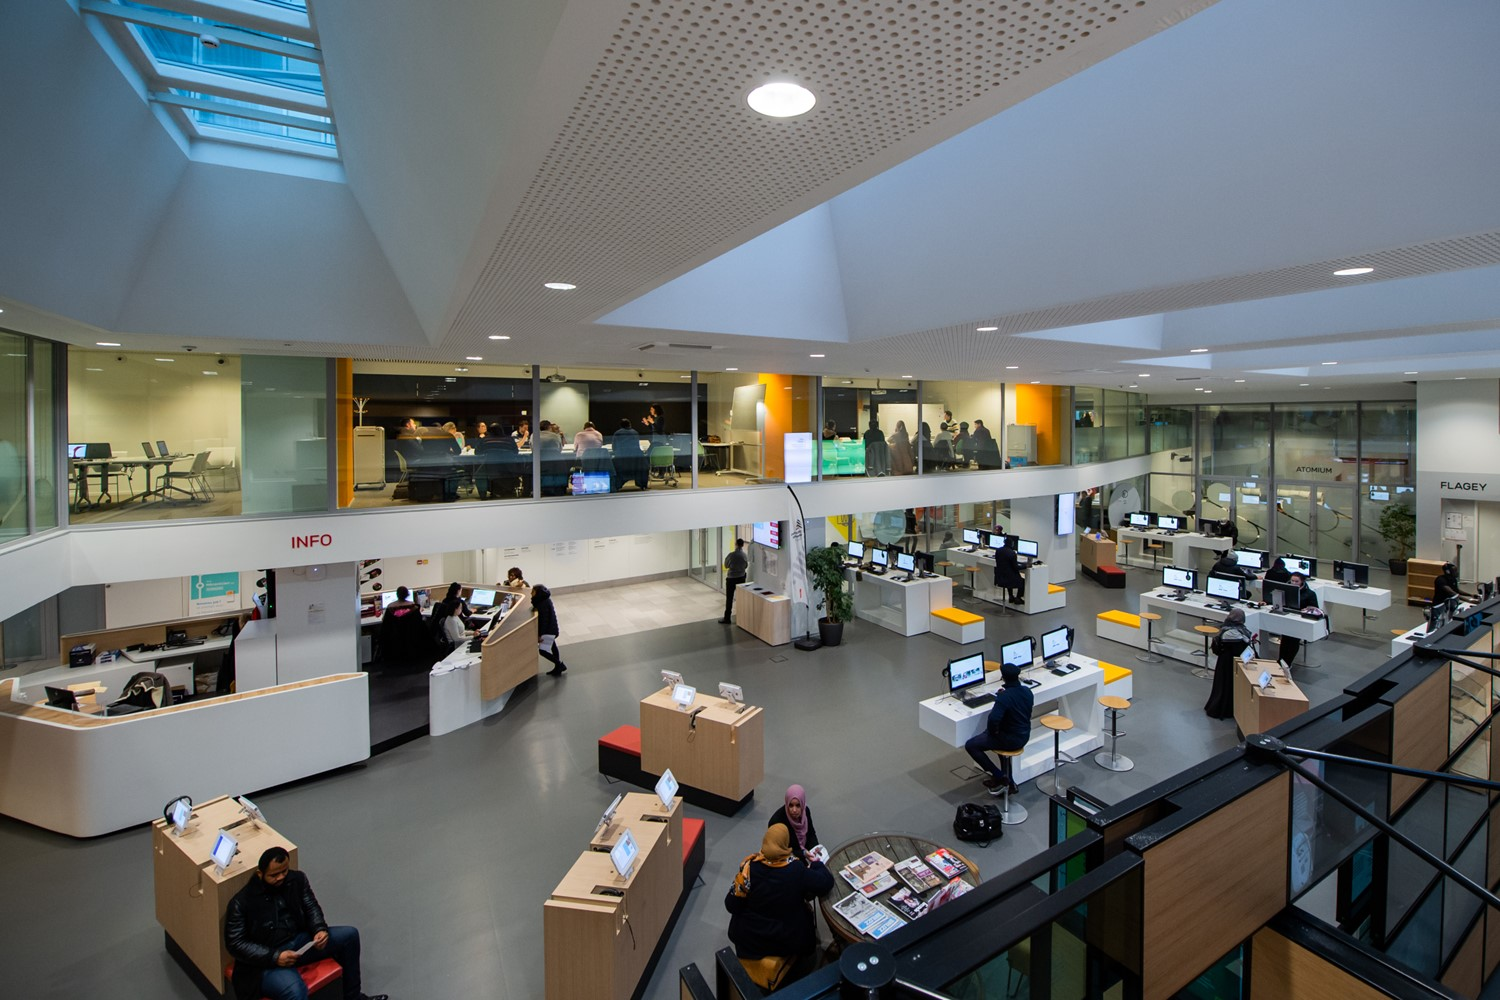
\includegraphics[scale=1]{imarina.JPG}
\caption{Vue d'ensemble de la Cité des métiers de Bruxelles (Source: xxxx)}
\end{center}
\end{figure}


\newpage
\subsection{Étude de Cas 2: Bibliothèque publique dans le nord-est du Nigeria \citep{Saleh}}
\quad Nous décrivons dans cette section les résultats de l'évaluation des services offerte par 06 bibliothèques publiques de l'État du Nord-est du Nigeria conduite par Adam Gambo Saleh et al. \\

\subsubsection{Enjeux de l'évaluation}
\quad C'est dans le but d'améliorer la qualité des services offerte par les bibliothèques publiques tout en impactant sur le développement éducatif de la région de Nord-est du Nigeria, que Adam Gambo Saleh et al. on évaluer les services de 6 bibliothèques publiques non seulement en mettant en lumière leurs faiblesses, mais aussi en apportant des solutions à celles-ci. Car depuis 1968 aucune étude n'avait été entreprise pour examiner la fourniture de services de bibliothèques publiques. \\

\subsubsection{Méthodologie}
\quad l'approche utilisée par les auteurs afin de mener cette étude a été l'évaluation quantitative à travers une méthode d'enquête au cours de laquelle deux instruments de travail ont été utilisés : 
\begin{enumerate}
\item[•]18 questionnaires soumis aux directeurs des conseils, responsables des divisions des services aux lecteurs et des services techniques des 06 bibliothèques.
\item[•]6 formulaires pour inventorier les ressources, les infrastructures et les équipements disponibles dans les bibliothèques étudiées.
\end{enumerate}

\subsubsection{Résultats}
\quad l'analyse des informations collectées a été faite grâce aux outils de la statistique descriptives qui ont permis aux chercheurs de structurer et de représenter information contenue dans les instruments d'évaluation à travers des tableaux, distribution de fréquences, des pourcentages, etc.
Il ressort de cette analyse qu'aucune des bibliothèques évaluer n'offre de services et support électroniques aux usagés; la raison évoquée est celle du manque d'équipements adéquate d'une part, d'autre part l'étude révèle que 3 services traditionnels sur 7 recommandés par l'IFLA/UNESCO ne sont pas fournis et la majorité des collections disponible son périmés, enfin les chercheurs ont noté aussi un manque de personnel adéquat et qualifié.\\
\subsubsection{Conclusion}
\quad En résumé, nous pouvons dire que l'approche d'évaluation utilisé dans le cadre de la présente étude de cas afin d'améliorer la qualité de service au sein des bibliothèques publique du Nord-Est du Nigeria est celle d'une approche ORIENTE EXPERT. D'après l'IFLA cette approche est la plus rependu au USA et est fondé sur les techniques et normes en vigueur au sein de la communauté professionnelle. Son principe se base d'une part sur les moyens nécessaire à l'adéquation des collections comme on peut le voir dans cette étude de cas ou près de 90\% des collections disponible dans les bibliothèque évalué étai périmé d'où l'inadéquation avec la politique envisager qui se voulait impacté sur le système éducatif du pays; d'autre part elle insiste sur les ressource nécessaire à la qualité de service et du personnel comme exemple, il en ressort de cette étude que le personnel de la bibliothèques étai peu qualifié ; et enfin son principe repose aussi sur le fait que les bâtiments doivent répondre à un certain standard. Outre cette approche l’IFLA présente aussi d'autre alternative à l'évaluation d'une bibliothèque\citep{noauthor_mesures_nodate} : 
\begin{enumerate}

\item[•]L'approche orienté objectif : 
Cette technique compare les résultats obtenus avec les objectifs fixé afin de déterminer la performance d'une bibliothèque dans l'atteinte de ces objectifs.

\item[•]L'approche orienté gestion : 
cette méthode est basée sur l'utilisation des indicateurs de tableau de bord afin d'orienté les prises de décision de gestion.  
\item[•]L'approche naturaliste et orienté participation :
Cette méthode est fondée sur l'identification des valeurs, critères, besoins et données avec l’implication des chaînes intervenantes (décideurs, employé, etc.). d'après l'IFLA elle guide actuellement les activités de recherche dans l'évaluation des projets de bibliothèque numérique. \\
\end{enumerate}
\quad comme limites a l'approche d'évaluation utilisé dans cette étude de cas, nous avons noté : 
\begin{enumerate}
\item[•] l'absence d'une évaluation centré sur l'usagé (client de la bibliothèque)qui pouvait être une enquête de satisfaction ou un entretien individuel afin de mieux cerné les besoins car a quoi bon avoir une collection de livre qui ne sont pas consulté si l'on veut avoir de l'impact sur un système éducatif du pays.
\item[•] on peut aussi remarqué l'absence de l'évaluation des bâtiment abritant la bibliothèque en termes de confort, de rayonnage et de luminaire. 
\item[•] ce même constat est aussi fait dans l'absence des propositions de méthodes marketing afin de booster les visites au sein de la bibliothèque car a quoi bon avoir des collections a jour s'il n'a personne pour consulter.
\end{enumerate} 

\newpage
\subsection{Étude de Cas 3}

\newpage
\section{Conclusion}






\newpage
\begin{center}
\listoffigures
\end{center}

\newpage

\begin{center}
\bibliography{bibliographie}
\bibliographystyle{unsrtnat} 
\end{center}

\end{document}
